\chapter{Estado de Arte}
\label{chap:estado-de-arte}
\section{Introducción general}
\label{sec:intro-general-qa}
Como vimos brevemente en la introducción, QA es un área de investigación de ciencias de la computación que busca generar respuestas concretas a preguntas expresadas en algún lenguaje natural. Es, por esto mismo, un problema complejo que involucra herramientas y modelos de otras áreas de existencia autónoma, como information retrieval (IR), procesamiento del lenguaje natural (PLN) e information extraction (IE).

También señalamos algunos ejes de subclasificación de problemas de QA. Con respecto al dominio de hechos y conocimientos sobre los que se espera que el sistema sepa responder, los sistemas se clasifican como de dominio abierto (\textit{open domain}) o de dominio cerrado (\textit{closed domain}): mientras de los primeros se espera que sepan responder preguntas acerca cualquier tema o dominio, de los segundos solo se espera que sepan responder preguntas acerca de un dominio acotado particular. A su vez, los datos pueden ser estructurados, semi estructurados o no estructurados. El ejemplo típico de una base de conocimientos estructurada es una base de datos relacional, un tipo de datos semi estructurados puede ser un documento XML no normalizado, mientras que el tipo de datos no estructurado por antonomasia es un corpus de documentos en texto plano.

Las bases de conocimiento de los sistemas de QA pueden tener uno o más tipos de datos, pero cada unos de estos tipos determina un enfoque algorítmico diferente. Por ejemplo, si la base de conocimientos es una DB relacional con un lenguaje formal de consultas similar al SQL, el problema de QA típico consiste en encontrar un mapeo desde la pregunta en lenguaje natural a una consulta formal expresada en un lenguaje comprensible para la base de datos. Esto implica que el foco de trabajo está en la generación de esta consulta y no en el trabajo posterior sobre los resultados de ejecutarla. Por otro lado, un corpus no estructurado no permite una consulta formal, por lo que el enfoque usual es obtener una lista de documentos relevantes para luego aplicar distintas técnicas de procesamiento de textos para extraer la respuesta buscada.

Estos dos ejes de clasificación (grado de especificidad del dominio y grado de estructuración de los datos) suelen tener una correlación, a saber: los dominios cerrados suelen disponer (o permitir la construcción sencilla de) una base de conocimientos estructurada, mientras que los dominios abiertos suelen forzar datos no estructurados. Esta correlación no es una asociación. En realidad, muchos sistemas open domain actuales son híbridos para estas clasificaciones, ya que suelen combinar varias bases de conocimiento de distintos tipos. Un sistema híbrido podría tener un corpora no estructurado basada en la web para preguntas generales y, a su vez, varias bases estructuradas para dominios específicos, que permiten responder sólo algunas preguntas con un resultado mejor. Otro uso puede ser extraer respuestas mediante métodos de PLN sobre corpora no estructurados para luego verificar su tipo contra bases de conocimiento estructuradas generales como Freebase o dbPedia.

En cuanto a aplicaciones comerciales masivas, podemos mencionar la aplicación Siri, el asistente personal de iOS y también la incorporación de funcionalidades de question aswering en los grandes buscadores\footnote{Buscar, por ejemplo: \dq{¿Cuándo nació Bill Gates?} en Google}.  Otros proyectos relativamente actuales que podríamos mencionar son Wolfram Alpha\footnote{\url{www.wolframalpha.com}}, un sistema online de question answering lanzado por la compañía Wolfram Research y también a IBM-Watson, el sistema de IBM que venció a los favoritos del show de trivia estadounidense Jeopardy!

La organización de este capitulo es como sigue: en lo que queda de esta sección (\allref{sec:intro-general-qa}), repasaremos la historia de la disciplina, desde sus orígenes hasta el estado actual de las competencias en torno a las cuales está hoy estructurada la investigación (\ref{subsec:historia}), luego reseñaremos las métricas utilizadas por estas competencias a la hora de evaluar la performance de los sistemas (\ref{subsec:metricas}). En la siguiente sección (\allref{sec:literatura}) pasaremos revista de diferentes investigaciones actuales sobre question answering para definir un modelo más o menos estándar del dominio de problemas y los acercamientos típicos, discutiendo diferentes investigaciones sobre QA open-domain (\ref{subsec:open-domain}), un enfoque estructurado para dominios cerrados (\ref{subsec:closed-domain}) y, finalmente el caso concreto de la implementación de IBM-Watson (\ref{subsec:ibm-watson}).


\subsection{Historia y Competencias}
\label{subsec:historia}
\label{subsec:competencias}
Los primeros sistemas que podemos considerar como pertenecientes al área datan de los años sesenta. Las primeras décadas de investigación al respecto están centradas en sistemas de dominio cerrado, es decir, su objetivo consiste en responder preguntas sobre temas específicos, apoyándose en general en una base de conocimientos estructurada, específicamente creada para el sistema. Por ejemplo Baseball \cite{BASEBALL}, un proyecto del MIT que data de 1961, es la primera investigación académica cuyo enfoque la incorpora con certeza en este área que pudimos encontrar en Internet. Baseball respondía preguntas sobre algunos hechos vinculados al torneo de la Liga Americana de baseball de un año concreto. La información se archivó de manera estructurada y contenía: el día, el mes, el lugar, los equipos y los puntajes de cada juego por un año\footnote{Como una nota de color, trascribimos las dos primeras oraciones del abstract: \dq{Baseball is a computer program that answers questions phrased in ordinary English about stored data. The program reads the question from punched cards.}. Traducido: Baseball es un programa de computadora que responde preguntas verbalizadas en inglés común sobre datos guardados. El programa lee la pregunta de tarjetas perforadas.}. Otro ejemplo conocido es el chatbot-psicóloga Eliza, cuyo código original fue escrito en 1966, que se basa en reglas muy simples de matcheo de las lineas ingresadas por el usuario para simular una conversación de terapia bastante convincente\footnote{En internet están disponibles diferentes implementaciones de Eliza. En \url{https://github.com/julian3833/eliza} puede encontrarse una implementación funcional en python}. Existieron otros desarrollos e investigaciones durante las siguientes décadas, con complejidad creciente, pero con un enfoque similar al de Baseball y de Eliza. Pero la investigación, la producción de software y, principalmente, la formación de una comunidad de desarrollo e investigación mínimamente articulada vinculada con el question answering estuvo impulsada fuertemente por el lanzamiento de los ejercicios de QA en la competencia TREC\footnote{\url{http://trec.nist.gov/}} (Text Retrieval Conference) en el año 1999, la TREC-8 \cite{TREC8}.

TREC se convirtió en una referencia obligada y centro de nucleamiento de la investigación en QA. Esta primera competencia mono-lengua (para inglés), consistía en retornar un fragmento de texto de entre 50 y 250 bytes conteniendo la respuesta a preguntas fácticas (factoids). La evaluación, que marcó la historia futura de la evaluación de QA en competencias, consideraba el sistema de QA como un todo, es decir, no consideraba la evaluación de subcomponentes. La organización permitía dar una lista con 5 respuestas posibles por cada pregunta, y esto siguió así hasta la TREC-2002, cuando se comenzó a exigir una sola respuesta por pregunta. TREC siguió lanzando un track de QA en todas sus competencias anuales, variando la forma y la complejidad de las tareas propuestas, por ejemplo: incorporando preguntas largas, con un formato realista y corpora de mayor tamaño, también introduciendo preguntas sin respuesta (NIL answers) y preguntas de tipo Lista (por ejemplo: \sq{¿Qué libros escribió Friedrich Nietzsche entre 1870 y 1896?}), pregunta de definiciones (por ejemplo: \sq{¿Quién es el General Paz?}), en TREC 2003, preguntas agrupadas por un tema (target), explícito o implícito y de diferentes tipos -como personas, organizaciones, cosas, eventos, etc-, restricciones temporales (por ejemplo: antes, durante y después de una fecha, evento o período), anáforas y co-referencias entre preguntas (por ejemplo: ¿Quién es George Bush?. ¿Y quién es \textit{su} esposa?), etc. Las competencias anuales de la TREC, por otro lado cambiaron el enfoque que existía en décadas anteriores, hacia preguntas de dominio abierto y corpora de datos textuales planos.

En lo que respecta a los sistemas multi-idioma (y mono-idioma no centrados en inglés), más allá de algunos eventos anteriores, un hito clave es el lanzamiento, en 2003, de la primer tarea de QA \cite{CLEF03} de CLEF (Cross Language Evaluation Forum)\footnote{\url{http://www.clef-initiative.eu/}} proponiendo tareas tanto monolingües como multilingües en varios idiomas europeos. Se propusieron tareas monolingües para francés, español, alemán, italiano y neerlandés, y tareas multilingües, con corpora en inglés y preguntas en otros idiomas europeos. En este año, se exigía respuestas de hasta 50 bytes, se permitía una lista de 3 respuestas por pregunta y las tareas podían incluir preguntas sin respuesta en los corpora. En la CLEF 2004, la tarea de QA principal incorporó 9 lenguas de origen (lengua de la pregunta) y 7 de destino (lengua del corpus), habilitando 55 ejercicios mono y bilingües. La cantidad de respuestas se redujo a 1 y se incorporaron preguntas de tipo \dq{¿Cómo...?}, de definiciones, de listas y también se agregaron restricciones temporales (antes, durante y después de una fecha, evento o período). En general, las respuestas concretas deben ir acompañadas de un fragmento de texto \dq{soporte}, es decir, el fragmento de texto del cual se extrajo la respuesta. CLEF continuó presentando {\em tracks} de tareas de QA todos los años desde entonces, con diferentes variaciones. Otra conferencia de prestigio en el área es NTCIR \footnote{\url{http://research.nii.ac.jp/ntcir/}}, que es un análogo a CLEF para idiomas asiáticos, incorporando tareas monolingües y bilingües entre inglés, japonés y chino, entre otras.

\subsection{Métricas de evaluación}
\label{subsec:metricas}

En cuanto a las métricas de evaluación utilizadas por estas competencias, es importante distinguir la evaluación de las respuestas a una pregunta y la evaluación general del sistema. Con respecto a la evaluación de respuestas, la clasificación usual de evaluación consiste en 4 valores asignados a cada respuesta: Correcta (C), si responde a la pregunta y el fragmento de soporte justifica esa respuesta; No soportada (U, de Unsupported), si responde a la pregunta pero el fragmento de soporte no está o no justifica la respuesta; Inexacta (X), si sobra o falta información en la respuesta (algunas competencias solo aceptan respuestas exactas) y, finalmente, Incorrecta (I), si ninguna de las condiciones anteriores se cumple.

La evaluación de respuestas puede ser estricta (strict) o \textit{indulgente} (lenient) dependiendo de si considera las respuestas no soportadas como válidas o como inválidas. Por otro lado, la evaluación puede ser manual -llevada a cabo por un jurado especial- o bien automática. En el caso de la evaluación automática, siempre es indulgente, ya que no hay forma automática sencilla de decidir si un fragmento soporta o no una respuesta. Para este tipo de evaluaciones se suele utilizar un set de patrones de respuestas correctas que se deriva de un set de \dq{respuestas conocidas} generadas por los organizadores y los mismos competidores, conocido como R-set, pero no es un proceso trivial: en principio, es difícil saber qué respuestas correctas pueden esperarse, ya que por la naturaleza del problema es probable que diferentes sistemas devuelvan respuestas textualmente distintas.

Con respecto a la métricas de evaluación para sistemas como un todo, veremos a continuación las métricas más conocidas: MRR (Mean reciprocal rank, o promedio de rankings recíprocos), CWS (Confidence Weighted Score, Puntaje ponderado por confiabilidad) y K-Measure (Medida K).

\subsubsection*{MRR - Mean Reciprocal Rank}
El MRR mide la habilidad de un sistema para responder un conjunto de pregunta $Q$. Asume que el sistema devuelve una o más respuestas por pregunta, en orden de \dq{confiabilidad}. El puntaje de cada pregunta individual ($RR(q_i)$) se define como la inversa de la posición de la primera respuesta correcta en la lista de respuestas dada, o cero si no hay ninguna.

\begin{equation}\label{eq:mrr}
 \text{MRR} = \frac{1}{|Q|} \sum_{i=1}^{|Q|} RR(q_i). \!
\end{equation}

\begin{equation*}
    RR(q_i) = \begin{cases}
               0     & \text{si no existe ninguna respuesta correcta}\\
               \frac{1}{\text{Posicion de }q_i} & \text{si }q_i\text{ es la primer respuesta correcta}\\
           \end{cases}
\end{equation*}

MRR puede tomar valores entre 0 y 1 inclusive, aunque el RR de cada pregunta tiene un espectro finito de valores (por ejemplo, para 5 respuestas puede valer 0, 0.2, 0.25, 0.33, 0.5 o 1). La primera vez que se usó MRR fue en la competencia TREC-8. En esa competencia se permitía una lista de 5 respuestas ordenadas para cada pregunta.


\subsubsection*{CWS - Confidence Weighted Score}
CWS (de Confidence Weighted Score, Puntaje de confiabilidad ponderada, también conocido como Precisión promedio) asume que el sistema devuelve una respuesta única por pregunta pero que estas respuestas a las diferentes preguntas están ordenadas por grado de confiabilidad descendente.
CWS recompensa respuestas correctas colocadas primero. CWS toma valores entre 0 y 1.  Uno de los principales problemas de esta métrica es que puede juzgar no la capacidad para responder preguntas sino la de ordenarlas por confiabilidad.

\begin{equation}\label{eq:cws}
 \text{CWS} = \frac{1}{|Q|} \sum_{i=1}^{|Q|} \frac{\text{Cantidad de rtas correctas en las primeras $i$ posiciones}}{i}. \!
\end{equation}


\subsubsection*{K-Measure}
K-Measure fue propuesta en \cite{CLEF04}. Pide a los sistemas una lista de respuestas por pregunta y un grado de confiabilidad para cada una de ellas, entre 0 y 1.

\begin{equation}\label{eq:k}
 \text{K} = \frac{1}{|Q|} \sum_{i=1}^{|Q|} \frac{\sum_{r \in ANS_i} conf(r) \times eval(r)}{\text{max}\{|R_i|, |ANS_i|\}}. \!
\end{equation}

Para una pregunta $i$, $R(i)$ es el total de respuestas distintas conocidas, mientras que $ANS_i$ son las respuestas dadas por el sistema a evaluar para la pregunta $i$, $conf(r)$ es la confiabilidad entre 0 y 1 asignada por el sistema a la respuesta $r$ y $eval(r)$ es la evaluación hecha por la organización.


\begin{equation*}
    eval(r) = \begin{cases}
               1  & \text{si $r$ es juzgada correcta}\\
               0  & \text{si $r$ está repetida}\\
               -1 & \text{si $r$ es incorrecta}\\
           \end{cases}
\end{equation*}

Vale que $K \in \mathbb{R} \wedge  K \in [-1,1]$ , y $K=0$ se identifica con un sistema que asigna confiabilidad 0 a todas sus respuestas y, por lo tanto sirve como baseline.

La dificultad principal de esta métrica es determinar un $R_i$ exhaustivo. Una propuesta alternativa que tiene esto en cuenta, propuesta también en \cite{CLEF04} es $K1$, que elimina la ocurrencia de $R_i$, pero solo sirve para evaluar sistemas que retornan una sola respuesta por pregunta.

\begin{equation}\label{eq:k1}
 \text{K1} = \frac{\sum_{r \in ANS_i} conf(r) \times eval(r)}{|Q|}. \!
\end{equation}

\begin{equation*}
    eval(r) = \begin{cases}
               1  & \text{si $r$ es juzgada correcta}\\
               -1 & \text{si $r$ es incorrecta}\\
           \end{cases}
\end{equation*}

Nuevamente, vale que $K1 \in \mathbb{R} \wedge  K1 \in [-1,1]$ y $K1=0$ se condice con un sistema sin conocimiento.

\section{Literatura y sistemas}
\label{sec:literatura}
% Estado: Agregar una introducción acá sobre qué veremos en esta sección.

\subsection{Enfoques sobre open domain}
\label{subsec:open-domain}
% Estado: limé aristas (brevemente) y eliminé la etiqueta \falta. Para el yo del 6-6 cuenta como Cerrado.
Existe un consenso general a la ahora de definir el modelo de software más abstracto o de arquitectura para encarar la construcción de un sistema de question answering open domain. Esta arquitectura consiste en un pipeline con al menos tres módulos o componentes bien diferenciados:
\begin{itemize}
\item Módulo de procesamiento de la pregunta
\item Módulo de procesamiento de documentos
\item Módulo de procesamiento de la respuesta
\end{itemize}

Cada uno de estos módulos cuenta a su vez con subcomponentes sobre los cuales hay mayor o menor consenso, que determinan, en definitiva, la performance del sistema concreto implementado.

El módulo de procesamiento de la pregunta tiene como subcomponente principal un Clasificador de Preguntas (Ver \allref{subsec:qc} y \allref{sec:stanford-qc}) y puede incorporar otros componentes como identificadores del \sq{foco} (\textit{focus}) y del tipo esperado de la respuesta (\textit{answer type}), y también puede incluirse en este módulo un componente encargado de expandir o reformular la pregunta para optimizar los resultados del módulo de procesamiento de documentos ( este subcomponente también se suele considerar como parte del módulo de procesamiento de respuestas). Este último subcomponente tiene diferentes nombres en la literatura (\textit{query reformulation}, \textit{query generation}, \textit{query expansion}, etc).

En el núcleo del módulo de procesamiento de documentos, por lo general, hay uno o más índices invertidos (por ejemplo, de Lucene o Indri) como el descripto en \allref{subsec:indice-invertido}, o bien accesos a un buscador web, o, más en general, estructuras de information retrieval. Como vimos (\ref{subsec:metricas-ir}), existen dos métricas fundamentales a la hora de evaluar el funcionamiento de un módulo de information retrieval: precisión y recall. La precisión es la proporción de documentos relevantes devueltos sobre el total documentos devueltos por el módulo, mientras que el recall es la proporción de documentos relevantes devueltos sobre el total de documentos relevantes existentes en la base de conocimientos. Estas dos métricas suelen comportarse una con la otra como un trade-off, es decir: suelen aparecer escenarios de diseño en los que se deberá optar por priorizar una o bien la otra. Considerando esto, existe una tercera métrica extendida, la medida $F$, que busca parametrizar este compromiso.

En el contexto de uso de los sistemas de QA, la métrica que se busca maximizar para el módulo de procesamiento de documentos es el recall, es decir, no interesa que el módulo no recupere documentos no relevantes siempre y cuando recupere todos los documentos relevantes existentes que pueda. El motivo es simple: se espera que el análisis lingüístico fino del módulo de procesamiento de la respuesta sea capaz de eliminar texto irrelevante en la misma o en mejor medida que el sistema de information retrieval subyacente al módulo de documentos. Por otro lado, si al recuperar los documentos se filtra una respuesta válida como irrelevante, entonces el resto del pipeline verá sus probabilidades de éxito mermadas (sino directamente anuladas).  La expansión/reformulación de la pregunta del paso anterior apunta, justamente, a generar una query que priorice el recall sobre la precisión.

Otras tareas que se realizan en el módulo de procesamiento de documentos es la división de los documentos en parágrafos, el filtrado de documentos o parágrafos irrelevantes y el ranking de los resultados. Si bien los sistemas de information retrieval suelen rankear sus resultados, este ranking puede resultar no del todo adecuado para la tarea en cuestión y mejorable teniendo en cuenta la información disponible.

Finalmente, el módulo de procesamiento de respuestas introduce el valor agregado que distingue un sistema de IR típico y un sistema de QA propiamente dicho. Este módulo es el menos estandarizado de los tres y tiene diferentes enfoques más o menos elaborados en la literatura, pero el grado de consenso sobre la viabilidad del uso de un grupo de técnicas fijas sobre otras no ocurre como, por ejemplo, en el uso de un clasificador de preguntas en el módulo de procesamiento de preguntas o de un índice de búsquedas en el módulo de procesamiento de documentos. Típicamente, el módulo consta de tres momentos:  a partir de los parágrafos o documentos rankeados generados por el módulo de documentos se busca identificar oraciones o respuestas candidatas mediante distintas técnicas. Para estas respuestas candidatas identificadas, se extrae la información concreta que responde a la pregunta utilizando heurísticas basadas en las etiquetas obtenidas para la pregunta (clase de pregunta, foco, tipo de respuesta, etc). Finalmente, se implementa algún mecanismo de corroboración o de validación de respuestas, generando una respuesta final.

A continuación nos extenderemos con más detalle sobre los tres módulos propuestos señalando algunos enfoques usuales, usando como guía los papers \cite{QA-survey}, \cite{QA1}, \cite{QA2}, \cite{QA3} y \cite{PASSAGE1}.

\subsubsection*{Módulo de procesamiento de la pregunta}
Este módulo recibe como input una pregunta formulada en algún lenguaje natural y genera como output una representación de la misma que resulte útil para los módulos siguientes. Esto suele realizarse agregando labels o etiquetas (ver detalle de \dq{Features}, en \allref{sec:terminologia}) a la pregunta completa y a sus distintos términos.

La etiqueta principal generada es el tipo de pregunta (\textit{question type}) y para obtenerlo se utiliza un clasificador como el que describimos en (\ref{subsec:qc})· Lamentablemente, la clasificación de preguntas no está desarrollada para otros idiomas que el inglés, al menos, no con el mismo grado de precisión y visibilidad que, por ejemplo, el clasificador de Stanford \cite{QC1} \cite{QC2}. Como vimos anteriormente, el principal problema a la hora de clasificar una pregunta es la ambigüedad intrínseca de ciertas clases de preguntas.

A partir del tipo de pregunta se define el tipo de respuesta esperada (\textit{answer type}). No existe un algoritmo automático estándar difundido para generar el tipo de respuesta esperado. El enfoque general encontrado es la aplicación de un mapeo simple basado en reglas, desde el tipo de pregunta generado por el clasificador a una serie de tipos de respuestas predefinido para el dominio de problema.

Otro análisis interesante pero, según nuestra investigación, no sistematizado, es el análisis del \dq{foco} (\textit{question focus}). En \cite{QA3} se define el foco como una palabra o secuencia de palabras que indican qué se está preguntando. Por ejemplo, para la pregunta \dq{¿Quién fue nombrado presidente de Argentina en  1983?} el foco sería \dq{presidente}). El concepto aparece también en \cite{WATSON1} pero no encontramos detalles sobre los mecanismos técnicos implicados en la extracción y todo parece señalar a una serie de heurísticas de procesamiento lingüístico escritas a mano.

Otros análisis que se realizan sobre la pregunta son el POS-tagging (Ver \allref{subsec:pos}), el reconocimiento de entidades nombradas (NER, ver \allref{subsec:nerc}) y la búsqueda de dígitos u otros patrones útiles para el contexto que excedan al NER.

Finalmente, se ejecuta la reformulación o expansión de la pregunta para genera un input para el módulo de information retrieval tal que maximice el recall.
La idea guía es la extracción de keywords relevantes y existen diferentes enfoques, usando los POS-tags y el resultado del NER. También pueden utilizarse recursos léxicos como Wordnet para generar sinónimos de términos importantes.

En \cite{QA1} y \cite{QA3} se propone una heurística basada en 8 reglas para implementar este paso. La implementación consiste en agregar, en orden, los siguiente tokens:

\begin{enumerate}
\item Seleccionar todas las palabras no stop words entre comillas
\item Seleccionar todas las entidades nombradas reconocidas
\item Seleccionar todas las construcciones nominales con sus adjetivos
\item Seleccionar todas las demás construcciones nominales
\item Seleccionar todos los sustantivos con sus adjetivos
\item Seleccionar todos los demás sustantivos
\item Seleccionar todos los verbos
\item Seleccionar el \sq{focus} de la pregunta
\end{enumerate}

\subsubsection*{Módulo de procesamiento de documentos}
El input del módulo de procesamiento de documentos es la pregunta reformulada según describimos en los párrafos inmediatamente anteriores y su output es una lista de documentos (o parágrafos) ordenados según la factibilidad de que contengan la respuesta a la pregunta. El módulo consta, en general, de uno o más sistemas de information retrieval (entre los cuales puede estar la web indexada) y de submódulos de filtrado, fragmentación y reordenamiento. Sobre los sistemas de information retrieval es importante notar que suelen usarse sistemas tradicionales y no aquellos como el utilizado, por ejemplo, en latent semantic analysis (LSA). Este último enfoque demostró ser útil a la hora de eliminar o reducir problemas de sinonimia y polisemia en information retrieval, pero en QA es importante que las keywords de búsqueda mismas estén presentes en los documentos relevantes y no que sean solamente \dq{semánticamente similares}. Dada la gran cantidad de documentos que se espera que retorne el subsistema de information retrieval (como señalamos, se prioriza el recall y no la precisión), existe un paso de filtrado (en \cite{WATSON1} se lo nombra como \sq{soft filtering}) en el cual: 1\textsuperscript{o} se reduce la cantidad de documentos a retornar por el módulo en general y 2\textsuperscript{o} se reduce la cantidad de texto en cada documento. El principio que guía este proceso es la idea de que las palabras clave de la pregunta deben aparecer, de alguna manera, cercanas entre sí. De este modo, es posible buscar por estas keywords en los documentos y quedarse solo con los $N$ parágrafos que contengas las keywords, desechando el resto del texto. Finalmente, se procede a ordenar los parágrafos/documentos filtrados. Una implementación posible de este ordenamiento es utilizar radix sort, considerando features de ordenamiento específicos para el dominio de problemas o bien re generando un índice de information retrieval con la nueva información recortada.


\subsubsection*{Módulo de procesamiento de la respuesta}
Finalmente, el módulo de procesamiento de respuestas es el encargado de generar una respuesta a partir del output de los otros dos módulos. Para ello debe identificar la respuesta dentro de los parágrafos, extraer la fracción de texto que responde puntual y concretamente a la pregunta y, finalmente, validar su corrección.

Para identificar la respuesta se utilizan distintas heurísticas, utilizando el tipo de respuesta esperado cuando es posible. Sin embargo, el tipo de respuesta esperado no siempre es explícito en la pregunta o en la respuesta, por lo que se utilizan diferentes reglas basadas en POS-tags, NERs, en un parser específico para el reconocimiento de las respuestas candidatas.

Para las respuestas candidatas se extrae luego el o los términos concretos de la respuesta final a partir del fragmento de texto elegido. Existe sobre este punto heurísticas más o menos avaladas basadas en distancias entre keywords, número de keywords presentes y otras métricas similares (veremos ejemplos de esto en la implementación de IBM y en el baseline de Qanus en breve). Típicamente, si no se encuentra ninguna coincidencia confiable, los sistemas de QA productivos recaen en la devolución de los primeros $n$ parágrafos mejor rankeados por el módulo de documentos.

Como señalamos anteriormente, en las competencias TREC hasta 2001 se permitía devolver una lista de 5 respuestas, mientras que desde el 2002 se exige una única respuesta.

Finalmente, hay distintas formas de validar la corrección o de estimar un grado de confianza en la corrección de una respuesta. Un enfoque típico es utilizar diferentes corpus específicos estructurados con los cuales contrastar la información obtenida hasta el momento. Veremos este enfoque en breve en \allref{subsec:ibm-watson}.

\subsection{QA como interfaz a una base de datos}
\label{subsec:closed-domain}
El enfoque a la hora de encarar una solución de question answering sobre dominios cerrados (específicos) difiere sustancialmente de los enfoques sobre dominios abiertos. Un dominio de conocimientos general fuerza datos en texto plano, documentos escritos en lenguaje humano, tal como vimos en la sección anterior. La razón de esto es que no existen bases de datos, o, en general, repositorios de datos estructurados acerca de... todo. En sistemas open domain, sin embargo, es posible incorporar bases de conocimiento estructuradas como complemento de otras no estructuradas. Cuando coexisten ambos tipos de datos, como vimos, hablamos de sistemas híbridos.

Los usos que puede hacer un sistema híbrido de sus bases de información estructurada son varios. Un uso típico es responder preguntas sobre dominios específicos, esto es, un sistema puede utilizar bases de conocimiento estructuradas y algoritmia específica para ciertos temas concretos (por ejemplo: Liga Americana del año 1958) y para ciertos tipos de preguntas (¿cuál fue el resultado del partido...?), mientras que para el resto de las preguntas recae en métodos de dominio abierto. Estos \dq{subsistemas} son más costosos y difíciles de construir, pero, en general, logran mejores resultados para las preguntas que acepta (y brindan una estimación de la confiabilidad de la respuesta bastante buena). Otro uso típico es verificar el tipo de una respuesta extraído de un corpus plano, contra ontologías como Freebase, Yago o dbPedia \cite{WATSON2}, por ejemplo, verificando que la respuesta generada para \dq{¿Quién fue el presidente de...?} sea una persona y, mejor, un presidente.

Los sistemas de dominio cerrado puros, por otro lado, tienen interés en diferentes ámbitos en los que se dispone de información estructurada de utilidad para crear una interfaz más natural con la DB, permitiendo así el acceso a la base de datos a personas sin los conocimientos técnicos necesarios para escribir una consulta en el lenguaje formal que brindan las bases de datos como interfaz de consultas.

Para ambos casos de uso de los modelos de dominio cerrado (sistemas híbridos y de dominio cerrado puros) el enfoque algorítmico consiste en traducir la pregunta formulada en un lenguaje natural a una consulta del lenguaje formal (potencialmente: SQL, SPARQL o similar). Dado que la cantidad de \dq{cuestiones} sobre las que se puede responder es siempre acotada, el modelo estándar de dominio cerrado sobre datos estructurados busca traducir la pregunta formulada en lenguaje humano a una consulta acerca de algún aspecto de la base de datos. Debe, además poder decidir si una pregunta tiene sentido en el contexto de la información de la que dispone.

%\subsubsection{Marco teórico utilizado en la tesis}

En esta tesis utilizamos como marco teórico el desarrollado por Ana-Maria Popescu et. al. en sus papers \cite{QADB1} y \cite{QADB2}.
% TODO: potencialmente, citar los otros trabajos que tengo en personal-folder/Thesis/

En estos trabajos, Ana María Popescu et. al. definen la noción de pregunta \textit{semánticamente tratable} en el contexto de una base de datos concreta. Proponen, así mismo, un modelo teórico para identificar este tipo de preguntas y una forma de transformarlas en consultas de SQL, así como también un sistema concreto que implementa el modelo, llamado PRECISE. Popescu argumenta que una interfaz a una base de datos en lenguaje natural puede no identificar una pregunta, pero que jamás debe mal interpretarla activamente, es decir, interpretar algo distinto a lo preguntado y dar una respuesta que no se condice con la necesidad de información del usuario. Una mala interpretación de una pregunta reducirá la confianza del usuario en el sistema, volviéndolo inusable. En cambio, identificando una pregunta como intratable, se puede disparar un proceso de reformulación o especificación asistida de la pregunta, lo cual no es tan costoso en términos de confianza en el sistema.

En lo que resta de esta sección, describiremos con detalle el modelo teórico propuesto por Popescu en sus publicaciones, así como también el sistema concreto implementado por sus autores con ese modelo como guía.

\subsubsection*{Definiciones iniciales: elementos, compatibilidad, token, correspondencia, tipado de tokens.}

Según el modelo relacional usual, una base de datos está compuesta de tres tipos de \textbf{elementos}: \textit{valores, atributos y relaciones}. Cada elemento es distinto y único. Por relación nos referimos a lo que usualmente llamamos tabla (por ejemplo: Universidades), por atributo a una columna de una tabla (por ejemplo: Dirección), y por valor a un dato particular de una fila de una columna (Por ejemplo: Figueroa Alcorta 1234).

Popescu define la noción de \textbf{compatibilidad} entre elementos como sigue:
\begin{enumerate}
  \item Un valor es compatible con su atributo
  \begin{itemize}
      \item Figueroa Alcorta 1234 es compatible con Dirección
  \end{itemize}
  \item Un valor es compatible con la relación que contiene a su atributo
  \begin{itemize}
    \item Figueroa Alcorta 1234 es compatible con Universidades
  \end{itemize}
  \item Un atributo es compatible con su relación
  \begin{itemize}
      \item Dirección es compatible con Universidades
  \end{itemize}
  \item Cada atributo tiene un conjunto de qwords compatibles
  \begin{itemize}
    \item Dirección es compatible con “Dónde”
  \end{itemize}
\end{enumerate}

Observemos que mientras las primeras tres reglas de compatibilidad son independientes de los contenidos de la base de datos, la cuarta, en principio, requiere una formulación explícita (humana) de la relación entre qwords y atributos.

Las \textbf{qwords}, recordemos, son los pronombres interrogativos, palabras típicas con las que comienza una pregunta: quién, qué, cómo, cuándo, dónde, etc para el castellano, why, where, who, which, etc para el inglés. En los trabajos de Popescu, se define extensivamente como una palabra dentro del conjunto \{what, which, where, who, when\}.

% TODO: Quizas, introducir que es un lema, pero qué sé yo
Por otro lado, se introduce una noción de \textbf{token}, diferente de la que dimos en \allref{sec:terminologia}.
En el contexto de este modelo, un token es un conjunto de lemas de palabras (Ver \allref{subsec:otras-tareas-pnl}) que corresponden a un elemento de la base de datos. Por ejemplo, \{experiencia, requerir\} y \{experiencia, necesario\} son tokens que corresponden al atributo “Experiencia Requerida” de una base de datos.

Otra definición inicial importante es el concepto de correspondencia\footnote{Traducimos aquí \textit{to match} por \textit{corresponder}}, que no está definido teóricamente sino operacionalmente al describir el sistema PRECISE. El procedimiento utilizado es el siguiente (Utilizaremos el atributo “Experiencia Requerida” como ejemplo para ilustrar cada paso):

\begin{itemize}
  \item Cada elemento de la base de datos se separa en palabras individuales:
  \begin{itemize}
    \item “Experiencia Requerida” $\rightarrow$ \{Experiencia, Requerida\}
  \end{itemize}
  \item Se genera un conjunto de sinónimos para cada palabra usando Wordnet:
  \begin{itemize}
    \item experiencia $\rightarrow$ \{experiencia, conocimiento, habilidad,...\}
    \item requerida $\rightarrow$ \{requerida, necesaria, indispensable,...\}
  \end{itemize}
  \item Se toman los lemas o raíces de todas las palabras
    \begin{itemize}
      \item experiencia $\rightarrow$ \{experiencia, conocimiento, habilidad,...\}
      \item requerida $\rightarrow$ \{requerir, necesario, indispensable,...\}
  \end{itemize}
  \item Se generan tokens combinando los lemas de los sinónimos de cada elemento:
  \begin{itemize}
      \item tokens = \{(experiencia, requerir), (conocimiento, requerir), (habilidad, requerir),(experiencia, necesario), (conocimiento, necesario), (habilidad, necesario),(experiencia, indispensable), (conocimiento, indispensable), (habilidad, indispensable)\}
  \end{itemize}
  \item Este conjunto de tokens se asocia a cada elemento:
  \begin{itemize}
    \item “Experiencia Requerida” $\rightarrow$ tokens (como está definido en el bullet anterior)
  \end{itemize}
\end{itemize}

Con este procedimiento se construye un diccionario de elementos de la base de datos en listas de tokens. Finalmente, basándose en este diccionario, se construye la función \textbf{correspondencia}, que va de tokens en elementos de la base de datos. Dado un token, se obtienen todos los elementos de la base de datos a los que ese token corresponde, esto es, todos los elementos para los cuales el token en cuestión pertenece al conjunto de tokens generado según el procedimiento recién enunciado. Notar que un token puede corresponder a más de un elemento de la base de datos.

Los tipos de elementos a los que un token corresponde determinan el conjunto de \textbf{tipos posibles de un token} dado: token de relación, token de atributo, token de valor. Qué tipo tome un token dentro de sus tipos posibles dependerá de la correspondencia utilizada en el contexto dado.


\subsubsection*{Tokenización completa, asociación sintáctica, traducción válida, tratabilidad semántica}

El conjunto de preguntas que este trabajo rescata como semánticamente tratables es un conjunto conceptualmente simple pero prácticamente muy abarcador. Esto significa que se abordan preguntas formuladas de forma sencilla, pero que corresponden a una gran cantidad de preguntas de las que realmente se deberá ocupar un sistema de interfaz en lenguaje natural a una base de datos. En cualquier caso, como ya dijimos antes, existe siempre la posibilidad de pedirle al usuario una reformulación de la pregunta. La definición de tratabilidad semántica se basa en -e intenta formalizar- la observación de que muchas preguntas formuladas en lenguaje natural constan de una especificación de pares atributo/valor así como también de valores sueltos, donde el atributo asociado está implícito. Por su parte, un atributo podría estar asociado, también a una qword.  Por ejemplo, consideremos la pregunta: “¿Qué carreras se dictan en universidades localizadas en Buenos Aires?” en el contexto de una base simplificada que conste de una sola relación Universidades con atributos (Nombre, Dirección, Director, Cantidad de Alumnos, Carreras). En este caso, la palabra “localizada” está relacionada con el atributo Dirección, y está asociada a los términos “Buenos Aires”, también relacionado con el atributo Dirección (como valor), el término universidades está relacionado con la relación Universidades, mientras que la qword “Qué” y el término “carreras” refieren, ambos, al atributo Carreras.

Para definir la tratabilidad semántica es necesario introducir antes dos definiciones más.

Considerando la definición de token recién enunciada, se define como una \textbf{tokenización completa de una pregunta \textit{q}} a cualquier conjunto de tokens en los que cada término no filtrado de $q$ aparece en exactamente un token del mismo. El filtrado de términos, por su parte, es uno de los primeros pasos del procesamiento en la implementación y, como veremos en la próxima sección, consiste en eliminar marcadores sintácticos y términos que no aportan información relevante a la pregunta. En el caso del ejemplo del párrafo anterior, serían los términos \dq{se}, \dq{dictan}, \dq{en}.

Por su parte, decimos que dos tokens están \textbf{sintácticamente asociados}\footnote{Traducimos aquí \textit{syntactic attachment} como \textit{asociación sintáctica}} en el contexto de una pregunta $q$ cuando estos dos tokens cumplen ciertas condiciones sintácticas en algún árbol sintáctico de la pregunta.
% Reemplacé "parse tree" por "árbol sintáctico y eliminé una referencia a una sección parse-tree"
La función $attachment$, que modela la asociación sintáctica, tiene como dominio un par de palabras o lemas (y la oración en la que aparecen) y como imagen Verdadero o Falso. En la implementación presentada por los investigadores (Precise), como veremos en la sección siguiente, se utiliza un Charniak Parser para modelar esta función.

Con estos conceptos definidos, podemos dar finalmente la definición de \textbf{traducción válida}\footnote{Traducimos aquí \textit{valid mapping} por \textit{traducción válida}}. Una traducción válida de una pregunta $q$ en un conjunto de elementos $E$ de una base de datos es una relación entre alguna tokenización completa de $q$ con elementos de $E$ que cumple las siguientes tres condiciones (notar que los términos \textit{correspondencia}, \textit{compatibilidad} y \textit{asociación sintáctica} están usados según las definiciones técnicas recién reconstruidas):
\begin{enumerate}
  \item Cada token se corresponde con un único elemento de $E$.
  \item Cada token de atributo se relaciona con un único token de valor, cumpliendo las siguientes condiciones:
  \begin{itemize}
    \item el atributo de la base de datos que corresponde al token de atributo y el valor de la base de datos que corresponde al token de valor son compatibles
    \item ambos tokens están sintácticamente asociados
   \end{itemize}
  \item Cada token de relación está relacionado a un token de atributo o bien a un token de valor, cumpliendo las siguientes condiciones:
  \begin{itemize}
    \item la relación de la base de datos que corresponde al token de relación y el elemento de la base de datos que corresponde al token de atributo o token de valor son compatibles
    \item ambos tokens (token de relación - token de atributo o bien token de relación - token de valor) están sintácticamente asociados
  \end{itemize}
\end{enumerate}

Notar que no se exigen condiciones sobre los tokens de valor (esto captura la intuición de que los valores pueden aparecer con su atributo asociado implícito).

Si una pregunta tiene al menos una traducción válida en la que todos los tokens son distintos y en la que al menos unos de sus tokens de valor es una qword, entonces la pregunta es \textbf{semánticamente tratable}.

Con estas definiciones queda definido el marco teórico necesario para el tratamiento de preguntas formuladas en algún lenguaje natural por un sistema de question answering estructurado: que una pregunta sea \textit{semánticamente tratable} significa que existe una traducción válida de los tokens significativos de la pregunta a elementos de la base de datos. Como veremos en la siguiente sección al exponer la implementación del sistema Precise, la traducción de elementos de la base de datos a una consulta para la misma es trivial.

\bigskip

Consideremos ahora, antes de discutir la implementación concreta propuesta pors los autores, dos ejemplos del procedimiento implícito en el marco teórico para la traducción de la pregunta en una serie de elementos de una base de datos.

En primer lugar, asumamos la base de datos con una única relación, Universidades, con atributos (Nombre, Dirección, Director, Cantidad de Alumnos, Carreras) y, como filas de la base de datos, una serie de universidades nacionales.

Consideremos ahora una posible construcción de tokens asociados a la relación (el término “Universidades”) y a los atributos - obviaremos la reconstrucción de los tokens para los posibles valores. Para la generación de sinónimos utilizamos aquí sinonimos.com.

\medskip

Universidades se lematiza como “Universidad” y tiene como sinónimos: \{universidad, facultad, colegio, instituto, academia\}.

Dirección es su propio lema y tiene tres acepciones con diferente sinónimos: \{1) consejo, enseñanza, orientación, tutela, guía, patrocinio, amparo, adiestramiento, 2) domicilio, residencia, localización, 3) rumbo, destino, camino, ruta, trayectoria, sentido, orientación, tendencia\}. Notar que la polisemia del término introduce un problema, dado que por contexto el único sentido - y los sinónimos asociados que nos interesaría conservar - es el 2) domicilio, residencia. En el paper no se hace hincapie en este problema. Una opción es realizar un filtrado de los sentidos a mano, lo cual puede ser una tarea tediosa y larga si el esquema de la base de datos es muy grande.

Para el caso de Cantidad de Alumnos, el procedimiento sugiere: primero, quitar “de”, luego generar sinónimos para las palabras Cantidad y Alumno (lema de Alumnos) y luego hacer una combinación de todos con todos. Para Cantidad obtenemos: \{cantidad, cuantía, suma, total, importe, coste, número, conjunto, tanto\}, para Alumno: \{alumno, estudiante, colegial, escolar, discípulo, becario\}. Entonces, los tokens para Cantidad de Alumnos serían: {(cantidad, alumno), (cantidad, estudiante), (cantidad, colegial), (cantidad, escolar), (cantidad, discípulo), (cantidad, becario), (cuantía, estudiante), (cuantía, colegial),...}.

Los tokens para Nombre, Director y Carrera pueden verse en la siguiente tabla.

\begin{center}
\begin{table}[h]
\centering
\begin{tabular}{| l |  p{12cm} |}
\hline
Elemento & Conjunto de tokens \\ \hline
Universidades &  universidad, facultad, colegio, instituto, academia\\ \hline
Nombre &  nombre, fama, nombradía, marca, membrete, firma, patronímico, apelativo, denominación, apellido, designación, apodo, alias\\ \hline
Dirección & dirección, consejo, enseñanza, orientación, tutela, guía, patrocinio, amparo, adiestramiento, domicilio, residencia, localización, rumbo, destino, camino, ruta, trayectoria, sentido, orientación, tendencia\\ \hline
Director & director, administrador, rector, jefe, presidente, encargado, dirigente, directivo, dignatario\\ \hline
Cantidad de Alumnos & Todas las combinaciones de un término de {cantidad, cuantía, suma, total, importe, coste, número, conjunto, tanto} con un término de {alumno, estudiante, colegial, escolar, discípulo, becario}\\ \hline
Carreras & carrera, corrida, carretilla, correteo, galopada, curso, trayecto, trayectoria, recorrido, camino, profesión, licenciatura, estudios, puesto, prueba competición, lucha, pugna\\ \hline
\end{tabular}
\caption{Tokens para la relación Universidades y sus atributos}
\label{table:temas}
\end{table}
\end{center}

Por otro lado, corresponde asociar a cada atributo y a cada relación, si tiene sentido, una lista de Qwords compatibles. Nosotros proponemos la siguiente relación de compatibilidad:

\begin{center}
\begin{table}[h]
\centering
\begin{tabular}{| l |  p{12cm} |}
\hline
Atributo & Conjunto de Qwords compatibles \\ \hline
Nombre &  Qué, Cuál\\ \hline
Dirección & Dónde\\ \hline
Director & Quién\\ \hline
Cantidad de Alumnos & Cuánto, Qué\\ \hline
Carreras & Qué \\ \hline
\end{tabular}
\caption{Compatibilidad de Qwords para los atributos}
\label{table:temas}
\end{table}
\end{center}

Consideremos ahora la pregunta utilizada anteriormente: “¿Qué carreras se dictan en universidades localizadas en Buenos Aires?”. En primer lugar, corresponde filtrar las palabras sin significado en nuestro contexto y lematizar el resto de las mismas: \{qué, carrera, universidad, localización, buen, aire\}.

Luego, tomamos estos términos y vemos a qué conjuntos de tokens pertenecen y, a partir de allí, a qué elementos de la DB pueden corresponderse.


A fines ilustrativos, asumimos que existe una universidad localizada en Buena Vista, Catamarca, para obtener una ambigüedad en un término.

\begin{center}
\begin{table}[h]
\centering
\begin{tabular}{| l | l |  p{8cm} | }
\hline
Término & Tokens & Elementos \\ \hline
Qué &  Qué - qword & Token de valor compatible con: Nombre (atributo), Cantidad de Alumnos (atributo), Carreras (atributo)\\ \hline
Carreras & carrera & Carreras (atributo) \\ \hline
Universidades &  universidad & Universidades (relación)\\ \hline
localizadas & localización & Dirección (atributo)\\ \hline
Buenos & (buen, aire), (buen, vista) & Buenos Aires (valor) y Buena Vista (valor)\\ \hline
Aires & (buen, aire) & Buenos Aires (valor)\\ \hline
\end{tabular}
\caption{Términos, tokens y elementos asociados}
\label{table:temas}
\end{table}
\end{center}

Existen, como puede verse, dos tokenizaciones: \{qué, universidad, localización, (buen, vista), (buen, aire)\} y \{qué, universidad, localización, (buen, aire)\}. Pero la primera no cumple la condición de que cada término debe aparecer en un solo token. Por lo tanto, la única tokenización completa en la que cada término aparece en uno y solo un token de la tokenización es la segunda.

Veamos ahora si, a partir de esta tokenización completa y su relación con elementos de la base de datos, podemos obtener una traducción válida.

Veamos las reglas:

\begin{enumerate}
  \item Cada token se corresponde con un único elemento de $E$.
  \begin{itemize}
      \item Esta regla se cumple para todos los tokens.
  \end{itemize}
  \item Cada token de atributo se relaciona con un único token de valor, cumpliendo las siguientes condiciones: 1) el atributo de la base de datos que corresponde al token de atributo y el valor de la base de datos que corresponde al token de valor son compatibles y 2) ambos tokens están sintácticamente asociados
  \begin{itemize}
    \item Tenemos dos tokens de atributos: localización y carrera y los tokens de valor son qué y (buen, aire). Debemos ver si localización y carrera se relacionan con alguno de los dos de la manera descripta. El atributo que corresponde a localización en la base de datos es Dirección, mientras que el valor que corresponde a (buen, aire) es \dq{Buenos Aires}, y ambos son compatibles (pues Buenos Aires es un valor del atributo Dirección). Por otro lado, la qword qué no es compatible con el atributo Dirección, que solo es compatible con la qword Dónde. Pasaremos por alto aquí la condición relativa a la asociación sintáctica por ser demasiado técnica (la veremos en las próximas secciones), pero baste decir que localización y (buen, aire) está sintácticamente relacionado según algún árbol sintáctico. Entonces, localización se relaciona con (buen, aire). Veamos ahora que carrera no se relaciona con (buen, aire), pues Carreras y \dq{Buenos Aires} no son compatibles, pero sí se relaciona con el token de valor \dq{qué}, por lo que esta condición se cumple.
   \end{itemize}
  \item Cada token de relación está relacionado a un token de atributo o bien a un token de valor, cumpliendo las siguientes condiciones: 1) la relación de la base de datos que corresponde al token de relación y el elemento de la base de datos que corresponde al token de atributo o token de valor son compatibles, 2) ambos tokens (token de relación - token de atributo o bien token de relación - token de valor) están sintácticamente asociados
  \begin{itemize}
    \item Solo hay un token de relación: universidad y es compatible con todos los tokens posibles (localización, carrera y qué) y tiene una relación sintáctica fuerte con localización, por lo que esta regla se cumple también.
  \end{itemize}
\end{enumerate}


Entonces, tenemos una traducción válida de la pregunta en elementos de la base de datos con par atributo-valor Dirección, Buenos Aires), el atributo Carreras asociado a una qword y la mención de la relación Universidades. Según el procedimiento que detallaremos en la próxima sección, esto implica que la pregunta “¿Qué carreras se dictan en universidades localizadas en Buenos Aires?” se traduce en la query: “SELECT Carreras FROM Universidades WHERE Direccion=\sq{Buenos Aires}”.



\subsubsection*{Implementación: Precise}

En esta sección describiremos la estructura general del modelo implementado en los trabajos citados y las soluciones dadas al problema de la traducción desde una tokenización completa a un conjunto de elementos y de este conjunto a una consulta computacionalmente tratable. En la implementación propia sobre la base de datos estructurada del proyecto Mitic, presentada en \allref{chap:4}, se podrá ver una implementación simplificada de este modelo.

El sistema consta de los siguientes módulos:
\begin{itemize}
  \item Lexicon: encargado de generar, para cada elemento de la base de datos, el conjunto de tokens sinónimos que se utilizará para verificar correspondencia.
  \item Tokenizer: encargado de generar todas las tokenizaciones completas de la pregunta y, para cada token, consultar al lexicon y retornar la lista de elementos de la base de datos que le corresponden.
  \item Matcher: encargado de verificar que las tokenizaciones completas y los elementos generados por el tokenizer cumplan las condiciones 1 a 3 utilizando un modelo de grafos y el algoritmo max-flow.
  \item Parser plug-in: el módulo computa la función de asociación sintáctica, basándose en el parse tree de Charniak.
  \item Query generator: dado el conjunto de elementos de la base de datos traducido de la pregunta, genera una query SQL.
  \item Equivalence Checker: verifica si diferentes queries son la misma formulada de diferentes maneras.
\end{itemize}

Comenzaremos describiendo las responsabilidades de cada módulo, para luego ver la interacción general de los mismos con un ejemplo tomado de \cite{QADB2}.

El Lexicon es un módulo que se construye offline, como una derivación de la base de datos, siguiendo el procedimiento enunciado en la sección anterior al describir la función de \textit{correspondencia}.
La interfaz del módulo, utilizada por el Tokenizador, consta de dos operaciones:
\begin{enumerate}
  \item Dado un lema, devolver el conjunto de tokens que lo contienen
  \item Dado un token, devolver el conjunto de elementos de la base de datos que le \textit{corresponden}, según la definición de correspondencia dada en la sección anterior de esta tesis.
\end{enumerate}

Para construir el lexicon a partir de la base de datos, se sigue el siguiente procedimiento: a cada elemento de la base de datos se le asocia un conjunto de lemas (este paso puede ser simplemente lematizando los términos o agregando, a mano, un \dq{conjunto aumentado} de lemas). A partir de estos lemas se construye una lista de sinónimos, utilizando una ontología (como, por ejemplo, Wordnet), obteniendo los sinónimos de cada palabra y luego generando los conjuntos de pares ordenados pertinentes (Ver el algoritmo en detalle en la sección anterior).

Por su parte, el Tokenizador es el punto de entrada del sistema. Recibe como input una pregunta en lenguaje natural y genera como resultado un conjunto de todas las posibles tokenizaciones completas de la misma. Para ello:
\begin{itemize}
  \item elimina los marcadores sintácticos,
  \item lematiza las palabras restantes
  \item para cada lema, consulta al Lexicon por el conjunto de tokens que lo contienen
  \item para cada token potencial, verifica que los demás lemas del token estén presentes en el conjunto de lemas
  \item para cada partición completa de los lemas en listas de tokens (es decir, para cada tokenización), busca los elementos de la base de datos que corresponden a cada uno de los tokens que la componen.
\end{itemize}

De este modo, el Tokenizador genera diferentes particiones del conjunto de lemas (tokenizaciones de $q$), cada una con una traducción de cada token a todos los elementos de la base de datos que le corresponden. Será responsabilidad del Matcher decidir que tokenizaciones completas son traducciones válidas.

El Matcher toma como input una tokenización completa de $q$, con todos los posibles elementos de la DB que corresponden a cada token. Más claramente:
\begin{itemize}
  \item Una lista de tokens en donde cada palabra de $q$ pertenece a un y solo un token
  \item Para cada uno de los tokens de la lista, un conjunto de elementos $E$ de la base de datos (los elementos que le \textit{corresponden}, en el sentido técnico de corresponder)
\end{itemize}

Este módulo es el encargado de verificar qué conjunto de elementos $E$ de entre los disponibles cumple con las condiciones semánticas 1 a 3 (de la definición de traducción válida). El problema es modelado como un problema de matching (apareamiento) de grafos y resuelto con un algoritmo de max-flow. Cada solución dada por el algoritmo es una posible interpretación semántica de la pregunta. Veremos el modelo y su funcionamiento al presentar el ejemplo en lo que sigue de esta sección.

El Matcher debe verificar, como parte de las condiciones, que ciertas palabras estén sintácticamente asociadas. Esta tarea es responsabilidad del módulo de Parsing (Parse plug-in). Internamente, este módulo utiliza un \textit{Charniak parser} para extraer relaciones entre palabras en la oración. Solo las traducciones que satisfagan las condiciones de asociación sintáctica son traducciones válidas.
%TODO Expandir charniak parser

Comenzaremos describiendo la interacción de los componentes desde una vista de alto nivel, basándonos en el ejemplo dado en el trabajo \cite{QADB1}, para luego entrar en más detalle a la implementación de cada módulo.

Consideremos la siguiente pregunta $q$, en inglés: \dq{What are the HP jobs on a Unix System?} en una base de datos simplificada con una sola relación \textit{Jobs}, con atributos (Description, Platform y Company).

El primer módulo que toma la pregunta como input es el Tokenizador. En primer lugar, se eliminan los marcadores sintácticos (Los \textbf{marcadores sintácticos} se definen como una lista de palabras, independientes de la base de datos, que no aportan información semántica a la pregunta. Este conjunto contiene lo que usualmente se define como \textbf{stop-words}\footnote{La traducción española de \textit{stop word} es \textit{palabra vacía}. Conservaremos en este trabajo el término inglés.}: artículos, pronombres, preposiciones y otras palabras funcionales que no aportan contenido). En este ejemplo, los marcadores sintácticos, como se puede ver en \ref{fig:popescu-example}, son un verbo y tres preposiciones: \textit{are, the, on, a}.

El resto de las palabras, lematizadas, son el conjunto: \textit{job, system, HP, Unix, what}. El Tokenizador busca para este conjunto, generar una tokenización completa de $q$, es decir, un conjunto de tokens en los que cada término de $q$ aparece en exactamente un token del conjunto y cada token corresponde a un y solo un elemento de la base de datos.

El \textit{Tokenizer}  produce una única tokenización completa de la pregunta: (what, HP, job, Unix, system).

\begin{figure}
  \centering
    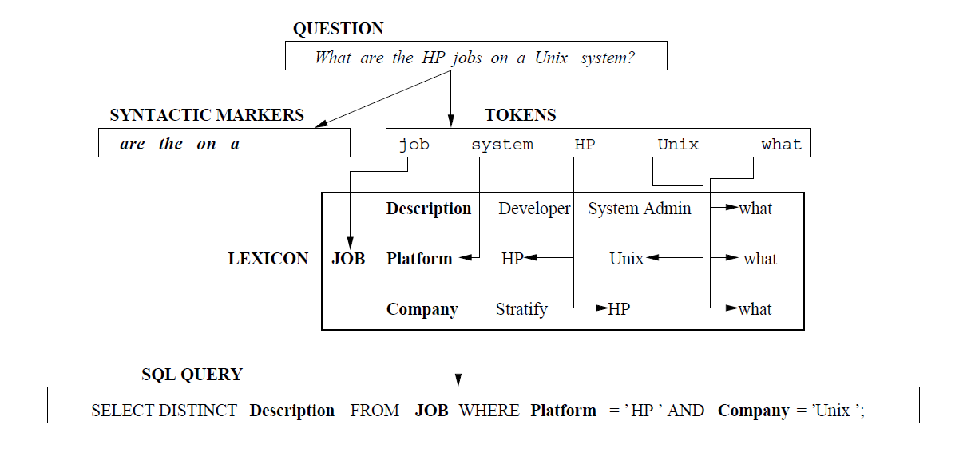
\includegraphics[scale=1.0]{graficos/popescu-example}
  \caption{Ejemplo de Popescu}
  \label{fig:popescu-example}
\end{figure}



Matcher.
Relaciones.

Alcance y limitaciones





%% Ver no se entiende mucho el ejemplo dado.
Ilustremos todos estos conceptos con un ejemplo: consideremos una base de datos $D$ con información sobre universidades y la siguiente pregunta $q$: \dq{¿Cuántos años tienen de docentes en estado activo que trabajan en la UBA?}, una traducción completa es el siguiente conjunto de \tradqd es: $\{\{\text{cuántos}, \text{años}, \text{tienen}\}_{attr=edad}, \{\text{docentes}\}_{rel=profesores}, \newline \{estado\}_{attr}, \{activo\}_{val}, \{trabajan\}_{attr=universidad}, \{UBA\}_{val=\text{Universidad de Buenos Aires}}\}$.

En esta traducción, quedan de lado las stopwords \{de, en, que, en, la\}, y se agrupan los tres primero tokens en la \tradqd\ $\{\{\text{cuántos}, \text{años}, \text{tienen}\}$ que mapea al atributo de $D$ \textit{edad}, y se mapea la \tradqd\ unitaria \{\dq{docentes}\} con la tabla \textit{profesores}, etc.



Por otro lado, es importante notar las limitaciones del modelo teórico recién expuesto. En principio, la navegación a través del modelo de datos no está contemplada y el manejo de relaciones se limita a relaciones de un grado.

En la próxima sección veremos un caso de éxito de un proyecto de question answering híbrido implementado por IBM y en el próximo capítulo describiremos la implementación de un modelo de question answering de dominio cerrado en el que utilizamos este marco como orientación.


\subsection{IBM-Watson}
\label{subsec:ibm-watson}
Watson\cite{WATSON1}\cite{WATSON2} es un sistema diseñado por IBM con el objetivo de competir en
tiempo real en el programa de televisión estadounidense Jeopardy,
logrando resultados del nivel de los campeones humanos de este
programa.

El proyecto demoró 3 años de investigación, en los cuales se
logró obtener la performance esperada (nivel humano experto) en
cuanto a precisión, confiabilidad y velocidad, logrando derrotar a
dos de los hombres con mayores récords históricos del show en un
programa en vivo\footnote{En esta url está disponible el programa en el que el sistema vence a sus competidores humanos: \url{http://www.youtube.com/watch?v=WFR3lOm_xhE}} en febrero de 2011.

El objetivo del \ proyecto puede considerarse una extensión de lo que
fue Deep Blue, el sistema que logró el nivel de los expertos humanos
en el ajedrez, porque buscó superar un reto  significativo y
visible del campo de la Inteligencia Artificial tanto para la comunidad
científica como para la sociedad en general:
{\textquotedblleft}?`puede un sistema computacional ser diseñado para
competir con los mejores hombres en alguna tarea que requiera altos
niveles de inteligencia humana y, si es el caso, qué clase de
tecnología, algoritmos e ingeniería se
requiere?{\textquotedblright} \cite{WATSON1}.

\medskip

A continuación presentamos brevemente la descripción de Watson según los trabajos \cite{WATSON1} y \cite{WATSON2}.

\medskip

Watson es la implementación específica para participar en este
programa de una arquitectura más genérica de question answering,
Deep-QA, que da el nombre al proyecto de la corporación. Esta
arquitectura es de construcción reciente y ejemplifica perfectamente la complejidad del problema de
QA de dominio abierto, incorporando tecnologías de punta de distintos
dominios de ciencias de la computación y de IA en particular:
information retrieval, natural language processing, knowledge
representation and reasoning, machine learning e interfaces humano -
computadora. En el transcurso de esta tesis, IBM lanzó el programa
\sq{Watson Ecosystem} (en noviembre de 2013) que promete la utilización
de tecnología de punta para aplicaciones creadas por la comunidad\footnote{
Announcing the IBM Watson Ecosystem Program: \url{http://www-03.ibm.com/innovation/us/watson/}}.

Watson debió cumplir con ciertas condiciones bastante exigentes, las que determinan su éxito como un real hito de question answering:


\begin{itemize}
\item Confiabilidad de la respuesta: \newline
Jeopardy tiene tres participantes con un pulsador y el que desee
responder debe pulsar antes que los demás. Además, existe una
penalización por respuestas incorrectas, por lo que es esencial que
el sistema pueda determinar la confiabilidad de la respuesta obtenida a
fin de optar por responder o no responder.
\item Tiempos de respuesta: \newline
La confiabilidad de la respuesta, o al menos una estimación, debe
calcularse antes de que pase el tiempo para decidir responder (6
segundos) y también de que otro participante oprima su pulsador
(menos de 3 segundos en promedio).
\item Precisión:\newline
El tipo de respuestas que se dan en el show suelen ser respuestas
exactas (por ejemplo: solamente un nombre, un número o una fecha,
etc).
\end{itemize}

\bigskip

El sistema tiene una arquitectura conocida como \sq{híbrida}, ya que cuenta con varios componentes heurísticos que estiman
ciertos features y grados de confiabilidad para diferentes respuestas, los cuales son evaluados por un sistema general que sintetiza un grado
de confiabilidad para una respuesta final y determina así si responder o no responder.

Jeopardy consta de un tablero con 30 pistas (o preguntas) organizadas
en seis columnas, cada una de las cuales es una categoría. Las
categorías van desde temas acotados como
{\textquotedblleft}historia{\textquotedblright} o
{\textquotedblleft}ciencias{\textquotedblright} hasta temas más
amplios como {\textquotedblleft}cualquier cosa{\textquotedblright} o
{\textquotedblleft}popurrí{\textquotedblright}. Watson intenta
respuestas sobre varias hipótesis de dominio y verifica en cual de
ellos se logran respuestas de mayor confiabilidad.

Por otra parte, el grueso de las preguntas de Jeopardy son del tipo
\textit{factoid}, esto es, preguntas cuya respuesta esta basada en
información fáctica acerca de una o más entidades individuales.

A su vez, existen ciertos tipos de pistas que requieren un enfoque
particular, por ejemplo, pistas que constan de dos subpistas muy
débilmente relacionadas, o problemas matemáticos formulados en
lenguaje humano, o problemas de fonética, etc, que no pueden ser
simplemente dejados de lado porque, si bien tiene poca probabilidad de
aparición, cuando aparecen lo hacen en bloque y pueden arruinar el
juego de Watson. Se acordó con la productora del programa, sin
embargo, dejar de lado preguntas audiovisuales (aquellas que presentan
una imagen o un audio y requieren interpretarlo) y preguntas que
requieren instrucciones verbales del presentador.


\bigskip

Para determinar el dominio de conocimiento, los investigadores analizaron 20000 preguntas, extrayendo su LAT (lexical answer type, o tipo léxico de respuesta). El LAT se define como una palabra en la
pista que indica el tipo de la respuesta esperado. Por ejemplo, para la pista {\textquotedblleft}Inventada en el Siglo XIV para agilizar el juego, este movimiento involucra dos piezas{\textquotedblright} el LAT es {\textquotedblleft}movimiento{\textquotedblright}. Menos del 12\% de las pistas no indicaba explícitamente ningún LAT, usando palabras
como {\textquotedblleft}esto{\textquotedblright} o {\textquotedblleft}eso{\textquotedblright}. En estos casos, el sistema debe inferir el tipo de respuesta del contexto. Del análisis de estas
20000 pistas se reconocieron 2500 tipos léxicos distintos, de los cuales los 200 más frecuentes no llegaban a cubrir el 50\% del total de pistas. Esto implica que un approach estructurado (orientado por el
tipo de respuesta), si bien resulta útil para algunos tipos, no es suficiente para abordar el problema completo.

\subsubsection*{Métricas}

Las métricas de resultados, además del tiempo de respuesta, son la
\textit{precisión} (preguntas contestadas correctamente / preguntas
contestadas) y el \textit{porcentaje de respuestas dadas }(preguntas
contestadas / total de preguntas). Mediante la configuración de un
threshold de \textit{confiabilidad} pueden obtenerse distintas
estrategias de juego: un umbral bajo repercutirá en un juego más
agresivo, incrementando la proporción de respuestas contestadas,
pero disminuyendo su precisión, mientras que un umbral alto
determinará un juego conservador, con menos respuestas dadas pero
mayor precisión en las mismas. Es un clásico escenario de trade-off
entre dos atributos de calidad. Un buen sistema de estimación de
confiabilidad implica una mejora general del sistema, aún cuando el
módulo de generación de respuestas permanezca idéntico.

En el show, el porcentaje de respuestas dadas depende de la velocidad
con la que se llega a presionar el pulsador, lo cual sólo interesa
para el dominio de QA como una restricción temporal.

Mediante análisis numérico, los investigadores determinaron que los
campeones de Jeopardy lograban tomar entre el 40\% y el 50\% de las
preguntas y, sobre ellas, lograban una precisión de entre el 85\% y
el 95\%, lo que determinaba una barrera de performance bastante
exigente en lo que respecta a QA.

\bigskip

\subsubsection*{Baseline}

El equipo de IBM intentó utilizar dos sistemas consolidados en QA y
adaptarlos al problema \ de Jeopardy. \ El primero fue PIQUANT
(Practical Intelligent Question Answering Technology), un sistema
desarrollado por IBM en conjunto con el programa del gobierno
estadounidense AQUAINT y varias universidades, que estaba entre los
mejores según la TREC. PIQUANT consta de un pipeline típico con
tecnología de punta, logrando un rango del 33\% de respuestas
correctas en las evaluaciones TREC-QA. Los requerimientos de la
evaluación de TREC son muy distintos de los de Jeopardy: TREC ofrece
un corpus de conocimiento relativamente pequeño (1M de documentos) de
donde las respuestas deben ser extraídas y justificadas, el tipo de
preguntas de TREC son menos complejas a nivel lingüístico que las
de Jeopardy y la estimación de confiabilidad no resulta una métrica
importante (dado que no hay penalización por respuestas incorrectas).
Además, los sistemas tienen permitido acceder a la web y las
restricciones temporales son, por mucho, más amplias (por ejemplo:
una semana para responder 500 preguntas). En Jeopardy, además de las
restricciones ya mencionadas, un requerimiento fue que el sistema
trabaje sobre datos locales y no acceda a la web en tiempo real. El
intento de adaptar PIQUANT al problema de Jeopardy dio pésimos resultados en
comparación con los necesarios: 47\% de precisión sobre el 5\% de
respuestas con mayor confiabilidad y 13\% de precisión en general.

Por otro lado, el equipo intentó adaptar el sistema OpenEphyra \footnote{\url{http://www.ephyra.info/}}, un framework open-source de QA desarrollado en
CMU (Carnegie Mellon University) basado en Ephyra (no libre), diseñado también para la evaluación TREC. OpenEphyra logra un 45\% de respuestas correctas sobre el set de datos de evaluación TREC
2002, usando búsqueda web. La adaptación resultó aún peor que la de PIQUANT (con menos del 15\% de respuestas correctas y una mala estimación de la confiabilidad).

Se probaron dos adaptaciones de estos sistemas, una basada en búsquedas de texto puro y otra basada en reconocimiento de entidades. En la primera, la base de conocimiento se modeló de manera no
estructurada y las preguntas se interpretaron como términos de una query, mientras que en la segunda se modeló una base de conocimientos estructurada y las preguntas se analizaron semánticamente para
reconocer entidades y relaciones, para luego buscarlos en la base. Comparando ambos enfoques en base al porcentaje de respuestas dadas, el primero dio mejores resultados para el 100\% de las respuestas,
mientras que la confiabilidad general era baja; por otro lado, el segundo enfoque logró altos valores de confiabilidad, pero sólo en los casos en que efectivamente logra identificar entidades. De aquí
se infiere que cada enfoque tiene sus ventajas, en el dominio de problemas apropiado.

\subsubsection*{La arquitectura DeepQA}
\label{subsec:deep-qa}
Los intentos de adaptación iniciales, como vimos, no dieron resultados, así como tampoco sirvieron las adaptaciones de algoritmos de la literatura científica, los cuales son realmente difíciles de
sacar de su contexto original y de las evaluaciones sobre las cuales fueron testeados. Como conclusión de estos intentos frustrados, el equipo de IBM entendió que una arquitectura de QA no debía basarse en sus componentes concretos sino en la facilidad para incorporar nuevos componentes y para adaptarse a nuevos contextos. Así surgió DeepQA, la arquitectura de base, de la cual Watson es una instancia concreta para un contexto particular (con requerimientos de alta precisión, buena estimación de confiabilidad, lenguaje complejo, amplitud de dominio y restricciones de velocidad). DeepQA es una arquitectura de cómputo paralelo, probabilístico, basado en recopilación de evidencia y scoring. Para Jeopardy se utilizaron más de 100 técnicas diferentes para analizar lenguaje natural, identificar y adjudicar valor a fuentes de información, encontrar y generar hipótesis, encontrar y rankear evidencias y mergear y rankear hipótesis en función de esta evidencia. La arquitectura sirvió para ganar Jeopardy, pero también se adaptó a otros contextos como la evaluación TREC, dando resultados mucho mejores que sus predecesores.
\medskip

A continuación, enumeraremos la lista de pasos que sigue el sistema para obtener la respuesta a una pregunta: \newline

\textbf{Adquisición de contenidos} \newline

El primer paso de DeepQA es la adquisición de contenidos. Este paso es
el único que no se realiza en tiempo de ejecución y consiste en
crear la base de conocimiento en la cual el proceso final buscará la
respuesta a la pregunta, combinando subprocesos manuales y
automáticos.

En principio se caracteriza el tipo de preguntas a responder y el
dominio de aplicación. El análisis de tipos de preguntas es una
tarea manual, mientras que la determinación del dominio puede
encararse computacionalmente, por ejemplo, con la detección de LATs
que señalamos antes. Dado el amplio dominio de conocimientos que
requiere Jeopardy, Watson cuenta con una gran cantidad de
enciclopedias, diccionarios, tesauros, artículos académicos y de
literatura, etc. A partir de este corpus inicial, el sistema busca en
la web documentos relevantes y los relaciona con los documentos ya
presentes en el corpus.

Además de este corpus de documentos no estructurados, DeepQA maneja
contenidos semi-estructurados  y estructurados, incorporando bases de
datos, taxonomías y ontologías como dbPedia, Wordnet y las
ontologías de Yago.\newline

\textbf{Análisis de la pregunta}\newline

El primer paso en run-time es el análisis de la pregunta. En este paso
el sistema intenta entender qué es lo que la pregunta está
formulando y realizar los primeros análisis que determinan cómo
encarará el procesamiento el resto del sistema. Watson utiliza
shallow parsers, deep parsers, formas lógicas, POS-tags,
correferencias, detección de entidades nombradas y de relaciones,
question classification, además de ciertos análisis concretos del
dominio del problema.

En este proceso se clasifica el tipo de la pregunta (los tipos están
determinados por el show: puzzles, matemáticos, etc). También se
busca el tipo de respuesta esperada, dónde los tipos manejados
por Watson son los LATs extraídos de las preguntas de ejemplo. El LAT
determina el {\textquotedblleft}tipo{\textquotedblright} de la
respuesta, qué clase de entidad \textit{es} la respuesta (una fecha, un
hombre, una relación, etc). El equipo de IBM intentó adaptar
distintos algoritmos de clasificación preexistentes, pero después
de intentar entrenarlos para el dominio de tipos de Jeopardy, llegaron
a la conclusión de que su eficacia era dependiente del  sistema de
tipos default, y que la mejor forma de adaptación era mapear su
output a los tipos utilizados por Watson (un enfoque similar fue
utilizado en esta tesis con respecto al clasificador de Stanford). Otra
anotación importante es el
{\textquotedblleft}foco{\textquotedblright} de la pregunta, la parte de
la pregunta tal que si se la reemplaza por la respuesta, la pregunta se
convierte en una afirmación cerrada.

Por ejemplo, para {\textquotedblleft}El hombre que escribió Romeo y
Julieta{\textquotedblright}, el foco es {\textquotedblleft}El hombre
que{\textquotedblright} (notar que esta definición de foco según los autores de IBM es diferente a la dada anteriormente en este capítulo). Este fragmento suele contener información
importante sobre la respuesta y al reemplazarlo por una respuesta
candidata se obtiene una afirmación fáctica que puede servir para
evaluar distintos candidatos y recolectar evidencia. Por ejemplo,
reemplazando por distintos autores y verificando que la oración
resultante esté presente en el corpus.

Por otro lado, muchas preguntas involucran relaciones entre entidades y,
más puntualmente, tienen una forma sujeto-verbo-objeto. Por ejemplo,
tomando la pista anterior, podemos extraer la relación
\textit{escribir(x, Romeo y Julieta)}. La amplitud del dominio de
Jeopardy hace que la cantidad de entidades y de relaciones entre
entidades sea enorme, pero esto empeora aún más al considerar las
distintas formas de expresar la misma relación. Por eso, Watson
sólo logra encontrar directamente una respuesta mediante
reconocimiento de entidades y relaciones sobre el 2\% de las pistas. En
general, este tipo de enfoque es útil sobre dominios más acotados,
mientras que la detección de relaciones como approach general a un
problema de question answering de dominio amplio es un área de
investigación abierta.

\medskip

\textbf{Generación de hipótesis}\newline

El tercer paso (segundo en run-time) es la generación de hipótesis:
tomando como input el resultado del paso anterior se generan respuestas
candidatas a partir de la base de conocimiento offline. Cada respuesta
candidata reemplazada por el foco de la pregunta es considerada una
hipótesis, que el sistema luego verificará buscando evidencias y
adjudicando un cierto grado de confiabilidad.

En la búsqueda primaria de respuestas candidatas, se busca generar
tantos pasajes como sea posible. El resultado final obtenido revela que
el 85\% de las veces, la respuesta final se encuentra entre los
primeros 250 pasajes devueltos por la búsqueda primaria. La
implementación utiliza una serie variada de técnicas, que incluyen
diferentes motores de búsqueda de textos (como Indri y Lucene),
búsqueda de documentos y de pasajes, búsquedas en bases de
conocimiento estructuradas como SPARQL con triple store y la
generación de múltiples queries a partir de una sola pregunta. La
búsqueda estructurada de triple stores depende del reconocimiento de
entidades y relaciones del paso anterior.

Para un número pequeño de LATs, se definió una suerte de conjunto
de entidades fijas (por ejemplo: países, presidentes, etc). Si la
respuesta final no es retornada en este paso, entonces no hay
posibilidad de obtenerla en los siguiente. Por eso se prioriza el
recall sobre la precisión, con el supuesto de que el resto del
pipeline logrará filtrar la respuesta correcta correctamente. Watson
genera varios cientos de hipótesis candidatas en este paso. \newline

Para optimizar recursos, se realiza un filtrado liviano (soft filtering) de respuestas
antes de pasar a la recopilación de evidencia y al scoring de
hipótesis. Un filtrado liviano es, por ejemplo, comprobar similaridad
de la respuesta candidata con el LAT esperado de la respuesta. Aquellas
hipótesis que pasan el filtro pasan al siguiente proceso, que realiza
un análisis más exhaustivo. \newline

\textbf{Recuperación de evidencias y scoring de pasajes}\newline

Para recuperar evidencias se utilizan varios algoritmos. Uno
particularmente útil es buscar la hipótesis candidata junto con las
queries generadas por la pregunta original, lo que señala el uso de
la respuesta en el contexto de la pregunta.  Las hipótesis con sus
evidencias pasan al siguiente paso, donde se les adjudica un score.

El proceso de scoring es donde se realiza la mayor parte del análisis
más fuerte a nivel computacional. DeepQA permite la incorporación
de distintos Scorers, que consideran diferentes dimensiones en las
cuales la hipótesis sirve como respuesta a la pregunta original. Esto
se llevó a cabo definiendo una interfaz común para los scorers.
Watson incorpora más de 50 componentes que producen valores y
diferentes features basados en las evidencias, para los distintos tipos
de datos disponibles (no estructurados, semi-estructurados y
estructurados). Los scorers toman en cuenta cuestiones como el grado de
similaridad entre la estructura de la respuesta y de la pregunta,
relaciones geoespaciales y temporales, clasificación taxonómica,
roles léxicos y semánticos que se sabe que el candidato puede
cumplir, correlaciones entre términos con la pregunta, popularidad (u
obscuridad) de la fuente del pasaje, aliases, etc.

Los distintos scores se combinan luego en un score único para cada
dimensión. \newline

\textbf{Merge y respuesta}\newline

Recién después de este momento, Watson realiza un merge entre
hipótesis idénticas. Las hipótesis idénticas son diferentes
formulaciones lingüísticas de lo mismo, por ejemplo:
{\textquotedblleft}X nació en 1928{\textquotedblright} o
{\textquotedblleft}El año de nacimiento de X es
1928{\textquotedblright}. Finalmente, se procede a estimar un ranking
único y una confiabilidad única para las distintas hipótesis. En
este paso se utilizan técnicas de machine learning que requieren
entrenamiento, y modelos basados en scores para ensamblar los distintos
resultados intermedios y generar una respuesta final.
